\documentclass{article}
\usepackage{amsmath} % for matrices
\usepackage{amssymb}
\usepackage{enumitem}
\usepackage{booktabs} % For better looking tables
\usepackage{graphicx} % For including images
\usepackage{caption}  % (Optional) For customizing captions
\usepackage{siunitx}
\usepackage{pdfpages}
\PassOptionsToPackage{hyphens}{url}\usepackage{hyperref}

\title{Baruch ML HW 6}
\author{Annie Yi, Daniel Tuzes, group 9}

\begin{document}
\maketitle

% insert table of contents here
\tableofcontents

\section*{Stock return classification}
In this exercise, we will collect financial data on various companies,
and potentially, further inputs that can affect stock prices to predict
whether a stock will go up, stay the same, or go down in the next period.

We then define a simple classification model,
the details of which we obtain from the Baruch ME pre-MFE course.
We label the data, train the model, and evaluate its performance.

Our goal is to show how a multi-dimenional,
multi-label classification problem
can be defined, trained, and used for prediction. Our hope to predict
market movement with any signicant accuracy is low.
    [But whou wouldn't want to be rich?]

\subsection*{Feature selection}
For brainstorming, we considered the features in the appendix.
We concluded in using the following features:

\begin{enumerate}
    \item The daily returns are used with different
          averaging windows. While the the weight within the
          window is constant, some more complicated averaging
          methods would be using decreasing weights as time
          difference increases. We can expact that if we went
          with a single averaged parameter, we would need to use
          a narrower window for daily return prediction,
          and a wider window for the monthly return prediction.

          We used a window size of 5 for daily and weekly returns,
          and window size of 3 for monthly returns. When calculating
          the weekly and monthly returns, we took the average over
          that time period, so the frequency of the data changed
          to weekly and monthly. This also means that the window size
          increased to 5 weeks and 3 months.
    \item Tha volatility is also used, where similarly,
          different prediction horizon required different
          time ranges. We took the sample's standard deviation
          over the same time windows as above.
    \item The trading volume is used, with the same
          considerations as above.
    \item As we were not familiar with technical indicators,
          we omitted them from our list.
    \item Price to earning is a widely used metric,
          and we incorporated it into our model. The earnings
          are reported quarterly, so we used the most recent
          value for every quarter, and using the daily returns.
    \item we selected stocks which pay little to no dividends,
          so we omitted the dividend yield.
    \item We considered the interest rate, however,
          we selected a time frame where the interest rate
          was constant low, so we omitted it.
          This raised a serious limitation on the training
          data, as the interest was low only between 2009 and 2015.
          To collect enough data, later we extended the time frame
          till 2022, when the interest rate was slightly elevated.
          See fig \ref{fig:interest} for the interest rate
          between 2009 and 2022.

\end{enumerate}

\begin{figure}[h]
    \centering
    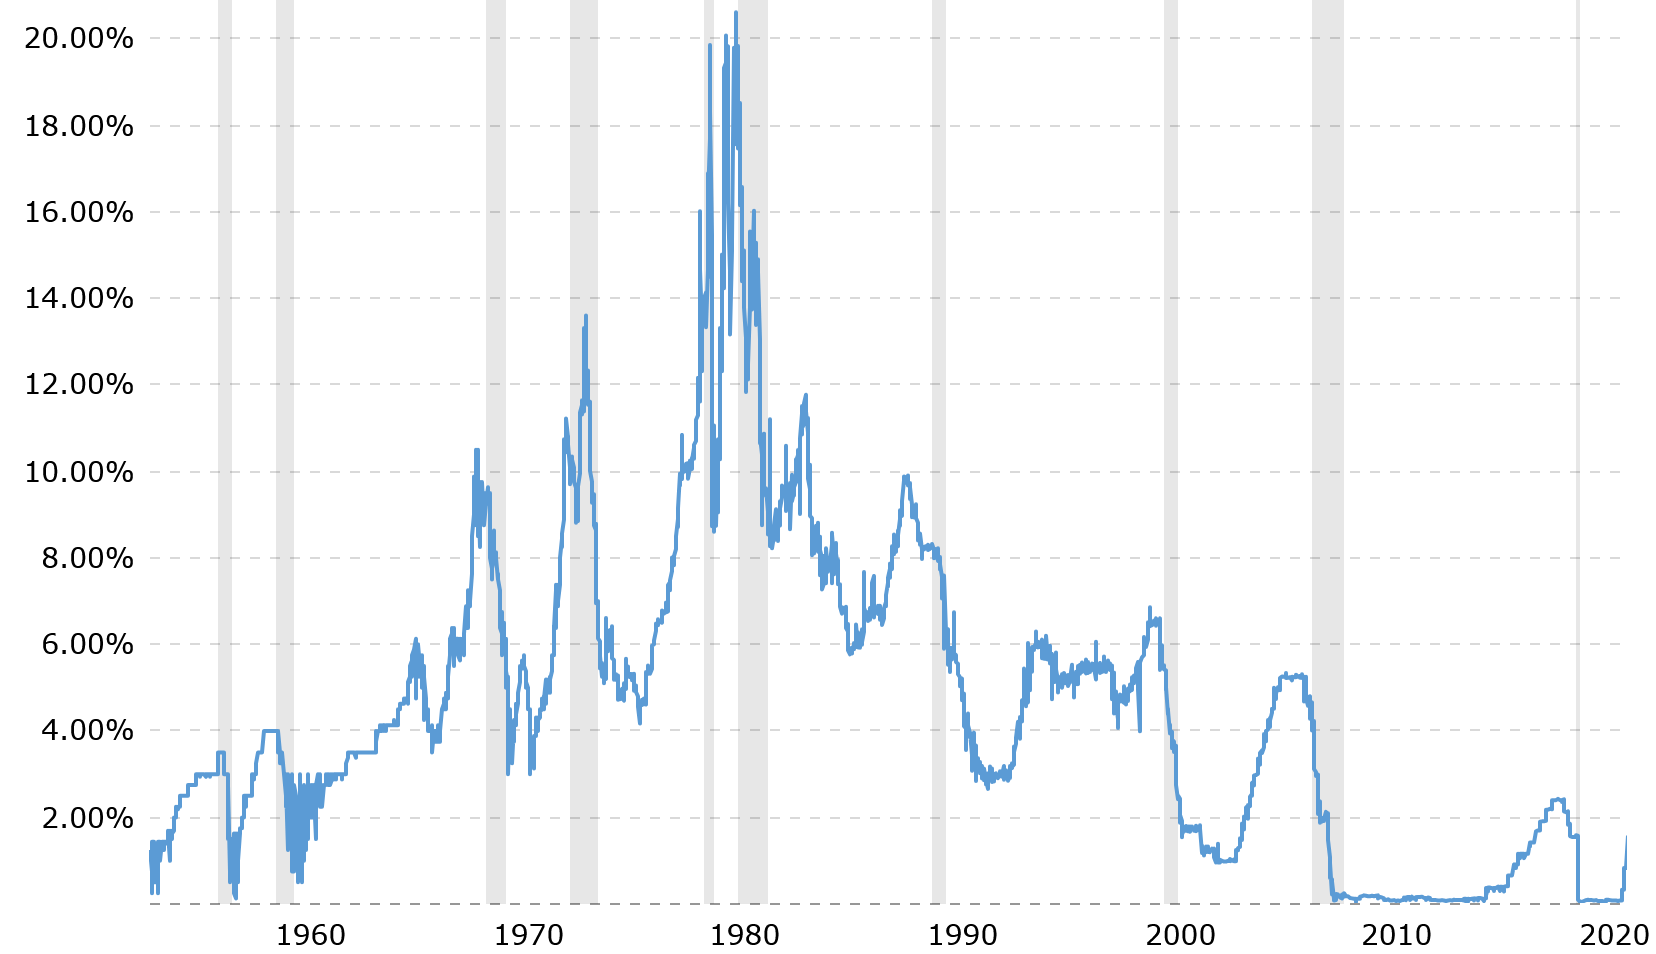
\includegraphics[width=0.7\textwidth]{IR.png}
    \caption{The interest rate between 2009 and 2022. Note that
        the interest rate was constant low between 2009 and 2015
        and slightly elevated between 2015 and 2022. Overall,
        the interest rate was low during this period compared
        to the historical average. Grey zones indicate recessions.
        Source: \url{https://www.macrotrends.net/2015/fed-funds-rate-historical-chart}}
    \label{fig:interest}
\end{figure}


\subsection*{Data collection}
We restrictred the model to features that are only stock specific.

\section*{Appendix}
\subsection*{Brainstorming on the list of features}

\small

Price-Based Features:

\begin{itemize}
    \item Daily Returns: The percentage change in stock price from one day to the next.
    \item Moving Averages: Simple Moving Average (SMA) and Exponential Moving Average (EMA) over different periods (e.g., 5-day, 10-day, 20-day).
    \item Volatility: Standard deviation of daily returns over a certain period. Relative Strength Index (RSI): Measures the speed and change of price movements.
    \item Bollinger Bands: Uses moving averages and standard deviations to identify overbought or oversold conditions.
\end{itemize}

Volume-Based Features:

\begin{itemize}
    \item Trading Volume: The number of shares traded in a given period.
    \item Volume Moving Averages: Similar to price moving averages but applied to trading volume.
    \item On-Balance Volume (OBV): A cumulative total of volume that adds or subtracts volume based on price movement.
\end{itemize}

Technical Indicators:

\begin{itemize}
    \item MACD (Moving Average Convergence Divergence): Shows the relationship between two moving averages of a stock’s price.
    \item Stochastic Oscillator: Compares a particular closing price of a security to a range of its prices over a certain period.
    \item Average True Range (ATR): Measures market volatility by decomposing the entire range of an asset price for that period.
\end{itemize}

Fundamental Features:

\begin{itemize}
    \item Earnings Reports: Quarterly earnings, earnings per share (EPS), and revenue growth.
    \item Financial Ratios: Price-to-Earnings (P/E) ratio, Price-to-Book (P/B) ratio, and Debt-to-Equity ratio.
    \item Dividend Yield: The dividend income relative to the stock price.
\end{itemize}

Macro-Economic Indicators:

\begin{itemize}
    \item Interest Rates: Changes in interest rates can affect stock prices.
    \item Economic Indicators: GDP growth rate, unemployment rate, and inflation rate.
\end{itemize}

Time-Based Features:

\begin{itemize}
    \item Day of the Week: Some stocks exhibit patterns based on the day of the week.
    \item Seasonality: Monthly or quarterly trends.
\end{itemize}


\end{document}
